%%%%%%%%%%%%%%%%%%%%%%%%%%%%%%%%%%%%%%%%%%%%%%%%%%%%%%%%%%%%%%%%%%%%%%
%%                     Logic arc
%%%%%%%%%%%%%%%%%%%%%%%%%%%%%%%%%%%%%%%%%%%%%%%%%%%%%%%%%%%%%%%%%%%%%%
%\color{blue}
\subsection{Glyph: \glyph{Logic arc} }\label{sec:logicArc}

\glyph{Logic arc} is used to represent the fact that an \corr{interactor}{\glyph{entity node}} \rougny{As defined in table 3.3.1} influences
the outcome of a \corr{logic operator}{\glyph{logical operator}}.

\begin{glyphDescription}
 \glyphSboTerm SBO:0000398 ! logical relationship.
 \glyphOrigin Any \corr{\glyph{interactor} (\sect{interactors}) or \glyph{logical operator} (\sect{logic})}{\glyph{entity node} (\sect{ENs})}.
 \glyphTarget Any \glyph{logical operator} (\sect{logic}).
 \glyphEndPoint No particular symbol is used to represent a logic arc.
 \end{glyphDescription}

\begin{figure}[H]
  \centering
  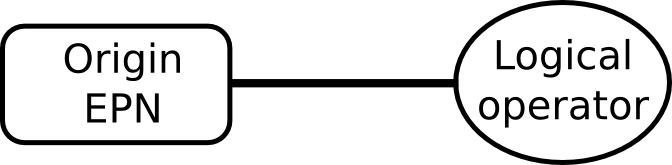
\includegraphics[scale = 0.4]{images/logicArc}
  \caption{The \ER glyph for \glyph{logic arc}.}
  \label{fig:logicArc}
\end{figure}

\begin{figure}[H]
  \centering
  \includegraphics[scale = 0.5]{examples/ex-logicArc}
  \caption{In this example, two logic arcs reflect the fact that the phosphorylation of threonine 306 on CaMKII is precluded either by a dimerisation or the binding of calmodulin.}
  \label{fig:ex-logicArc}
\end{figure}

%\normalcolor
